% --------------------------------------------------
% Delegation cascades: why safe instructions produce unsafe agents
%
% Venue-neutral: single column, standard article class, numbered references.
%
%   pdflatex main && bibtex main && pdflatex main && pdflatex main
% --------------------------------------------------
\documentclass[11pt,a4paper]{article}

\usepackage[T1]{fontenc}
\usepackage[utf8]{inputenc}
\usepackage{lmodern}
\usepackage[margin=1in]{geometry}
\usepackage{graphicx}
\usepackage{amsmath,amssymb,amsthm}
\usepackage{booktabs}
\usepackage{caption}
\usepackage{float}
\usepackage[section]{placeins}
\usepackage{authblk}
\usepackage[numbers,sort&compress]{natbib}
\usepackage{microtype}
\usepackage{tikz}
\usetikzlibrary{arrows.meta,positioning,calc,decorations.pathmorphing}
\usepackage{xcolor}          % must precede hyperref: allcolors uses a mixed colour
\usepackage[colorlinks=true,allcolors=blue!55!black]{hyperref}

\captionsetup{font=small,labelfont=bf,width=\textwidth}
% keep floats near the text that refers to them
\renewcommand{\topfraction}{0.92}
\renewcommand{\bottomfraction}{0.75}
\renewcommand{\textfraction}{0.07}
\renewcommand{\floatpagefraction}{0.80}
\setcounter{topnumber}{3}
\setcounter{bottomnumber}{2}
\setcounter{totalnumber}{4}
\setlength{\parskip}{0pt}
\renewcommand{\baselinestretch}{1.15}

\newtheorem{theorem}{Theorem}
\newtheorem{proposition}[theorem]{Proposition}
\newtheorem{lemma}[theorem]{Lemma}
\newtheorem{corollary}[theorem]{Corollary}
\theoremstyle{definition}
\newtheorem{definition}[theorem]{Definition}
\newtheorem{remark}[theorem]{Remark}

\definecolor{cAS}{HTML}{0072B2}
\definecolor{cCS}{HTML}{009E73}
\definecolor{cCAS}{HTML}{E69F00}
\definecolor{cAU}{HTML}{D55E00}
\definecolor{cGrey}{HTML}{4D4D4D}

\newcommand{\AS}{\textsf{AS}}
\newcommand{\CS}{\textsf{CS}}
\newcommand{\CAS}{\textsf{CAS}}
\newcommand{\AU}{\textsf{AU}}
\newcommand{\piP}{\pi_{P}}
\newcommand{\piS}{\pi_{S}}
\newcommand{\R}{\mathbb{R}}

\title{\bfseries Delegation cascades: why safe instructions\\ produce unsafe agents}

\author[1]{Author One}
\author[1,2]{Author Two}
\affil[1]{Affiliation One}
\affil[2]{Affiliation Two}
\date{}

\begin{document}
\maketitle

\begin{abstract}
\noindent
We study what happens to a safety instruction when it is passed down a chain of
delegated agents before anything is done with it. A principal enters a
competitive race but does not act in it: it issues a specification to an agent,
which issues one to a sub-agent, and so on for $d$ hand-offs. Two things happen
along the chain, and both are geometric in $d$. The specification is
transmitted imperfectly, so it survives $d$ hand-offs intact with probability
$(1-\varepsilon)^{d}$. Responsibility is traced back only in part, so a
principal at depth $d$ is charged the fraction $\phi^{d}$ of the harm it causes.
We embed both in the reduced four-strategy AI race of Fern\'andez Domingos and
Han, make delegation depth part of the strategy, and analyse the resulting
dynamics. Four results follow. First, depth is an unbounded liability shelter.
Realised harm saturates while attributed harm decays, so for every $\phi<1$
there is a depth beyond which each further hand-off strictly lowers the bill
even though it strictly raises the damage. No level of liability stops chains
from lengthening past it. Second, and against the intuition that the two
mechanisms simply add up, neither is dangerous on its own. Start from a race
that liability has already made safe at depth zero. Imperfect transmission alone
lifts the long-run unsafe frequency to $0.018$ and imperfect attribution alone
to $0.012$; together they lift it to $0.322$, so $91\%$ of the joint effect is
an interaction. A counterfactual that freezes the population composition
isolates its single cause. Under full pass-through the market answers
transmission loss by \emph{shortening} its chains, from six hand-offs to two,
and per-layer attribution is precisely what disables that answer. Third, the
resulting equilibrium is one in which every principal issues the safest
available instruction and the population executes the unsafe designs anyway:
declared and executed behaviour differ by $0.74$ in total variation. Fourth,
instruments that act on the incentive to delegate behave monotonically while
instruments that act on transmission fidelity do not. A partial fidelity
improvement can leave the ecosystem worse off than no improvement at all,
because over-specification was an equilibrium response to erosion. A ceiling of
one hand-off removes the unsafe behaviour entirely and raises social payoff from
$-0.8$ to $60.5$.
\end{abstract}

\noindent\textbf{Keywords:} evolutionary game theory; delegation; principal-agent
chains; liability; AI governance; multi-agent systems

\section{Introduction}
\label{sec:intro}

Software that acts on behalf of someone else is increasingly built as a chain.
A person instructs an agent, the agent decomposes the task and instructs
sub-agents, and the sub-agents call further tools and agents. The process that
finally takes an action in the world is then several hand-offs away from the
party that wanted it taken~\citep{wu2023autogen,park2023generative}.
Governance of such systems is written almost entirely at the two ends of the
chain. Safety training and evaluation act on the model; liability, procurement
rules and disclosure requirements act on the principal. The hand-offs in
between are treated as plumbing.

They are not plumbing. A hand-off does two things that matter. It transmits a
specification imperfectly, because each layer restates the task in its own
terms and the part most easily dropped is the qualifying clause rather than the
task itself. Degradation under repeated re-encoding is a robust property of
transmission chains, in human cultural transmission~\citep{kirby2008cumulative}
and in recursive machine generation~\citep{shumailov2024collapse}. And it
attenuates responsibility, because harm that reaches the world through several
intermediaries is traced back to the party at the top only in part. Both
effects are per-layer, so both compound geometrically with the number of
hand-offs. What is not obvious is what a population of principals does about
them.

The question matters because the two effects push the principal in opposite
directions. Imperfect transmission is a private cost: a principal who is held
responsible for what its chain does has every reason to keep the chain short.
Imperfect attribution is a private benefit: depth buys a discount on the bill.
Which force wins is not a matter of taste. Neither is the answer to the policy
question that follows: whether an instrument that improves transmission, one
that restores attribution, or one that simply caps the length of the chain does
more for the same effort.

We answer both by making delegation depth a strategic variable in an
evolutionary model. The interaction layer is the reduced four-strategy AI race
of~\citet{domingos2026falling}, used without modification, so that every depth
effect we report is attributable to the delegation layer we build on top of it.
A design is a pair $(d,s)$: a number of hand-offs and the specification the
principal issues. One hand-off acts on the specification by a row-stochastic
kernel, and the harm a chain causes is charged to its principal at the rate
$\phi^{d}$. Principals do not optimise; designs that pay better are copied
more, in the standard replicator and finite-population dynamics of evolutionary
game theory~\citep{taylor1978ess,hofbauer1998evolutionary,traulsen2006stochastic}.

Our contribution is an explanation, not a method or a benchmark. In one
sentence: \emph{delegation depth is a strategic variable whose two effects are
individually minor and jointly decisive, because per-layer attribution disables
the market's own response to specification erosion.} The results below make
that precise.

\paragraph{Results.}
We show, first, that depth is an unbounded liability shelter
(Theorem~\ref{thm:shelter}). Realised harm saturates in $d$ because the specification is eventually
forgotten, while attributed harm carries the extra factor $\phi$ per layer. For
every $\phi<1$ there is therefore a depth beyond which each further hand-off
strictly reduces the harm the principal is charged for while strictly increasing
the harm it causes. Beyond that depth the invasion
condition for one more layer stops depending on liability in the usual
direction: raising the penalty makes the deeper design \emph{more} attractive,
not less (Proposition~\ref{prop:invasion}).

Second, the two mechanisms do not add. We calibrate the liability so that the depth-zero race is already safe: the
effective liability we use is $3.1$ times the level at which the single-layer
game has long-run unsafe frequency zero. At that setting, imperfect
transmission alone yields $0.018$ and imperfect attribution alone yields
$0.012$, while the two together yield $0.322$. The interaction,
$+0.293$, is $91\%$ of the joint effect. A counterfactual that holds the population composition fixed shows why. Under
full pass-through the population answers transmission loss by shortening its
chains from six hand-offs to two. That answer, and not any change in behaviour
at a given depth, is what per-layer attribution removes.

Third, the equilibrium that results is one in which safety declarations are
uninformative. Every principal issues \AS{}, the safest available
specification, and the population executes \AS{} only $26\%$ of the time; the
distance between what is declared and what is executed is $0.74$ in total
variation. Over-specification is the equilibrium response to erosion, and it
does not repair it.

Fourth, the four governance instruments we compare are not
interchangeable. Restoring attribution has a threshold rather than a gradient:
nothing happens until $\phi$ reaches $0.86$, after which chains collapse from
six hand-offs to two. Capping chain length is monotone and cheap, and a ceiling
of one hand-off both removes the unsafe behaviour and raises social payoff from
$-0.8$ to $60.5$. Improving transmission fidelity is neither monotone nor safe in the small.
Taking the erosion probability from $0.20$ to $0.07$ reduces the unsafe
frequency to $0.032$, but taking it to $0.04$ raises it again to $0.239$,
because the improvement removes the reason principals were over-specifying. Where a single check is placed in the chain matters by a
factor of $18$, and it should be placed at the agent that acts.

\paragraph{Assumptions.}
Three should be stated at the outset rather than at the end. The chain
transmits one specification per race, so the executed designs of the two seats
are independent draws and every payoff is bilinear; a model in which layers
re-negotiate during play would not have this structure. The erosion kernel is
exogenous and is not itself under selection, so we describe what a market does
under a given transmission technology, not how that technology evolves. And
attribution decays geometrically, which is a modelling choice that we treat as
the definition of per-layer liability rather than as an empirical claim;
Section~\ref{sec:limitations} reports what changes when it is replaced.

\section{Related work}
\label{sec:related}

\paragraph{Evolutionary models of AI races.}
The idea of treating a development race between AI teams as an evolutionary
game is due to~\citet{han2020regulate}. The reduced four-strategy race we use as
our interaction layer is the model of~\citet{domingos2026falling}, in which
participants repeatedly choose Safe or Unsafe, unsafe development pays more per
round and advances faster, and a leader who cut corners carries a private risk
of a setback. That line of work has since examined regulation,
voluntary commitments and monitoring as ways of moving the
equilibrium~\citep{han2026trust}. All of it places the strategic agent in the
race. Our contribution is orthogonal: we leave the race exactly as it is and
ask what happens when the party whose design is being selected is several
hand-offs removed from the party that acts.

\paragraph{Delegation to artificial agents.}
Behavioural work has shown that delegating a decision to an artificial agent
changes what people choose, sometimes towards more prosocial
outcomes~\citep{domingos2022delegation}. That literature studies a single
delegation step, from a human to a machine. The governance literature has begun
to describe multi-step agentic delegation and the accountability problems it
raises~\citep{hammond2025multiagent,agentic2026governance,delegation2026intelligent},
but as far as we are aware without a formal model in which the depth of the
chain is itself selected. Making depth a strategic variable is what allows the
two mechanisms to be separated and their interaction to be measured.

\paragraph{Hierarchies, control loss and responsibility.}
That authority degrades as it passes down a hierarchy is a classical
observation in the economics of organisation. It appears as the loss of control
that bounds firm size~\citep{williamson1967hierarchical}, as the cost of
decentralised information processing~\citep{radner1993organization}, and as
collusion between layers~\citep{tirole1986hierarchies}. Diluted responsibility
in teams is equally classical~\citep{holmstrom1982moral}, and the law has long
recognised that liability must sometimes be assigned to a party other than the
actor for incentives to survive an
intermediary~\citep{shavell1980strict,sykes1984vicarious}. Our model brings the
two together and adds the ingredient those literatures do not have: a
population in which the depth of the hierarchy is not chosen by an optimising
designer but selected by differential replication of designs.

\paragraph{Specification and alignment.}
The gap between a stated objective and an executed one is the subject of the
specification-gaming literature~\citep{amodei2016concrete}, and incomplete
contracting has been proposed as the right frame for
alignment~\citep{hadfieldmenell2019incomplete}. Those accounts locate the gap
between the principal and a single agent. We locate a second gap, which
compounds with the number of intermediaries and which no amount of care at
either end of the chain removes.

\section{Model}
\label{sec:model}

\subsection{The interaction layer}

Two seats play the repeated race of~\citet{domingos2026falling}. In each round
a seat plays Safe or Unsafe. Unsafe pays more in the stage game, with round
payoffs $1.0$ and $0.6$ for a safe player against a safe and an unsafe
opponent against $2.4$ and $2.0$ for an unsafe one, and it contributes $1.5$
rather than $1$ to race progress. The race lasts $T$ rounds, with $T$
guaranteed to be at least five and stopping with probability $0.2$ per round
thereafter, so $\mathbb{E}[T]=9$. The leader in accumulated progress at the
horizon takes a prize of $100$, split on a tie, and a seat that is at risk
loses everything it has accumulated with probability $p_{\max} n^{U}/T$, where
$n^{U}$ is its number of unsafe rounds and $p_{\max}=0.6$.

Following the source study we work with four reduced designs, written here in
the order in which their specifications lose clauses:
\AS{} is unconditionally safe, \CS{} opens Safe and then copies the opponent,
\CAS{} opens Unsafe and then copies, and \AU{} is unconditionally unsafe. All
four are deterministic, so the action path of an ordered pair is fixed once
the pair is fixed and the only stochastic primitive is the horizon. We
therefore evaluate every matchup by exact expectation over the horizon law
rather than by sampling, which removes simulation noise from the payoff matrix
entirely. Write $a(i,j)$ for the expected task payoff of design $i$ against
$j$, $m(i,j)$ for its expected number of Unsafe actions and $u(i,j)$ for its
expected fraction of Unsafe rounds.

% generated by scripts/run_analysis.py -- do not edit
\begin{table}[t]
\centering
\caption{Interaction layer at depth zero. Task payoff $a(i,j)$ and expected number of Unsafe actions $m(i,j)$ of the focal design $i$ against $j$, evaluated exactly over the horizon law. Reading down a column, $m$ never falls: the erosion order is a harm order.}
\label{tab:race}
\begin{tabular}{lrrrrrrrr}
\toprule
& \multicolumn{4}{c}{$a(i,j)$} & \multicolumn{4}{c}{$m(i,j)$} \\
\cmidrule(lr){2-5}\cmidrule(lr){6-9}
$i$ & AS & CS & CAS & AU & AS & CS & CAS & AU \\
\midrule
AS & 59.00 & 59.00 & 8.60 & 5.40 & 0.00 & 0.00 & 0.00 & 0.00 \\
CS & 59.00 & 59.00 & 26.64 & 16.60 & 0.00 & 0.00 & 4.22 & 8.00 \\
CAS & 101.77 & 61.63 & 27.20 & 27.20 & 1.00 & 4.78 & 9.00 & 9.00 \\
AU & 48.64 & 47.36 & 27.20 & 27.20 & 9.00 & 9.00 & 9.00 & 9.00 \\
\bottomrule
\end{tabular}
\end{table}

\begin{table}[t]
\centering
\caption{The two mechanisms, separately and together. Long-run Unsafe frequency $U$, mean delegation depth $\bar{d}$, declaration gap and social payoff in the stationary regime of the finite-population process. Neither mechanism does much alone; the interaction is 0.293, or 91\% of the joint effect.}
\label{tab:decomposition}
\begin{tabular}{llrrrr}
\toprule
erosion $\varepsilon$ & attribution $\phi$ & $U$ & $\bar{d}$ & gap & $\pi_S$ \\
\midrule
$0$ & $1$ & 0.0000 & 6.00 & 0.000 & 68.0 \\
$0.2$ & $1$ & 0.0176 & 1.99 & 0.358 & 58.3 \\
$0$ & $0.75$ & 0.0115 & 5.95 & 0.000 & 65.5 \\
$0.2$ & $0.75$ & 0.3225 & 6.00 & 0.738 & -0.8 \\
\midrule
\multicolumn{2}{l}{interaction} & +0.2934 & & & \\
\bottomrule
\end{tabular}
\end{table}

\begin{table}[t]
\centering
\caption{Depth ceilings. Long-run Unsafe frequency and social payoff when chains longer than $\bar{D}$ hand-offs are forbidden. The social payoff is maximised well inside the ceiling the market selects.}
\label{tab:cap}
\begin{tabular}{lrrr}
\toprule
$\bar{D}$ & $U$ & $\bar{d}$ & $\pi_S$ \\
\midrule
0 & 0.0000 & 0.00 & 59.0 \\
1 & 0.0000 & 1.00 & 60.5 \\
2 & 0.0178 & 2.00 & 58.3 \\
3 & 0.0640 & 3.00 & 49.9 \\
4 & 0.1359 & 4.00 & 36.0 \\
5 & 0.2251 & 5.00 & 18.5 \\
6 & 0.3225 & 6.00 & -0.8 \\
\bottomrule
\end{tabular}
\end{table}



Reading down any column of $m$ in Table~\ref{tab:race}, the entries never fall.
This monotonicity is the structural fact on which everything below rests, and we
record it as a property of the interaction layer rather than an assumption of
ours.

\begin{lemma}[The erosion order is a harm order]
\label{lem:order}
For every opponent $j$, $m(\AS{},j)\le m(\CS{},j)\le m(\CAS{},j)\le m(\AU{},j)$,
and the same holds for $u$. The property is verified numerically for every
prize in $\{50,100,200\}$ and every $p_{\max}$ in $\{0.1,0.3,0.6,0.9\}$.
\end{lemma}

\subsection{The delegation chain}

A seat is operated not by a principal but by a chain
\[
  \text{principal} \;\longrightarrow\; \text{agent}_1 \;\longrightarrow\;
  \cdots \;\longrightarrow\; \text{agent}_d \;\longrightarrow\; \text{the race},
\]
where $d\ge 0$ is the \emph{delegation depth}. The principal issues one
specification, its \emph{intent} $s$, and each hand-off transmits it through
the row-stochastic kernel
\begin{equation}
  M \;=\; (1-\varepsilon)\,I \;+\; \varepsilon\,D ,
  \label{eq:kernel}
\end{equation}
with $\varepsilon$ the per-hand-off erosion probability and $D$ a drift kernel
on the four designs. The identity term in~\eqref{eq:kernel} is the part of a
specification that survives a hand-off untouched. Our baseline $D$ is the \emph{ladder}: an erosion event
moves the specification one rung down the order \AS{}, \CS{}, \CAS{}, \AU{},
which is to say it drops one safety clause and leaves the description of the
task intact. Two alternatives are used as controls. Under \emph{collapse} an
erosion event discards the specification and the sub-agent falls back on the
locally competitive design \AU{}. Under \emph{uniform} it replaces the
specification with a uniformly random one; that kernel has the same spectral
gap as the ladder but no direction, and it separates the effect of biased
erosion from the effect of noise as such.

The executed design of a depth-$d$ chain with intent $s$ is therefore
distributed as row $s$ of $M^{d}$, written $p_{d,s}$. Figure~\ref{fig:schematic}
shows the construction, and Figure~\ref{fig:transmission} shows what it does
to an \AS{} instruction.

\begin{figure}[t]
\centering
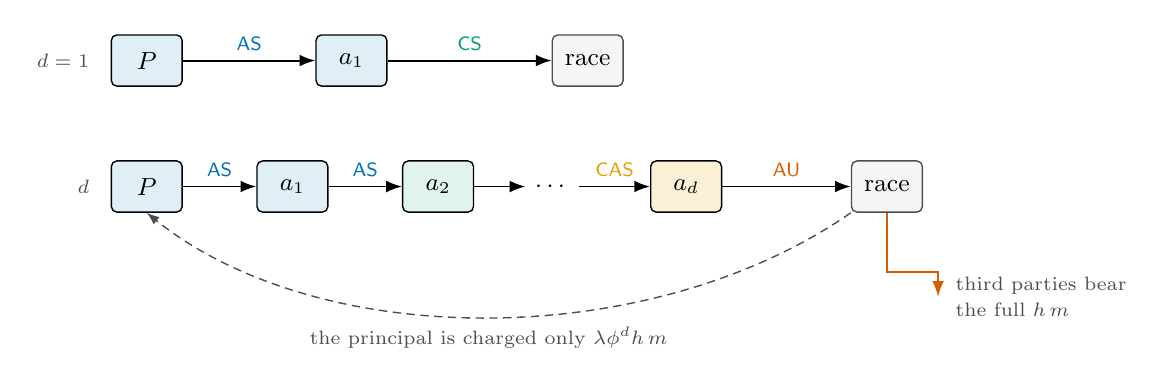
\begin{tikzpicture}[
  font=\small,
  box/.style={draw,rounded corners=2pt,minimum height=6.5mm,minimum width=9mm,
              inner sep=2pt,line width=0.5pt},
  spec/.style={font=\scriptsize\sffamily},
  flow/.style={-{Latex[length=2mm]},line width=0.7pt},
  faint/.style={-{Latex[length=1.6mm]},line width=0.5pt,densely dashed,cGrey}
]
% ---- shallow chain
\node[box,fill=cAS!12] (p1) at (0,2.15) {$P$};
\node[box,fill=cAS!12] (a1) at (2.6,2.15) {$a_1$};
\node[box,draw=cGrey,fill=black!4] (r1) at (5.6,2.15) {race};
\draw[flow] (p1) -- node[spec,above,text=cAS]{\AS} (a1);
\draw[flow] (a1) -- node[spec,above,text=cCS]{\CS} (r1);
\node[left=1.5mm of p1,font=\scriptsize,text=cGrey]{$d=1$};

% ---- deep chain
\node[box,fill=cAS!12] (p2) at (0,0.55) {$P$};
\node[box,fill=cAS!12] (b1) at (1.85,0.55) {$a_1$};
\node[box,fill=cCS!12] (b2) at (3.7,0.55) {$a_2$};
\node[font=\small] (dots) at (5.15,0.55) {$\cdots$};
\node[box,fill=cCAS!16] (b6) at (6.85,0.55) {$a_d$};
\node[box,draw=cGrey,fill=black!4] (r2) at (9.4,0.55) {race};
\draw[flow] (p2) -- node[spec,above,text=cAS]{\AS} (b1);
\draw[flow] (b1) -- node[spec,above,text=cAS]{\AS} (b2);
\draw[flow] (b2) -- (dots);
\draw[flow] (dots) -- node[spec,above,text=cCAS]{\CAS} (b6);
\draw[flow] (b6) -- node[spec,above,text=cAU]{\AU} (r2);
\node[left=1.5mm of p2,font=\scriptsize,text=cGrey]{$d$};

% ---- consequences
\node[align=left,font=\scriptsize,text=cGrey,anchor=west] (world) at (10.15,-0.85)
     {third parties bear\\ the full $h\,m$};
\draw[flow,cAU] (r2.south) -- ++(0,-0.75) -| (10.05,-0.85);
\draw[faint] (r2.south west) .. controls (6.4,-1.55) and (2.2,-1.55) ..
     node[font=\scriptsize,below,text=cGrey,pos=0.5]
     {the principal is charged only $\lambda\phi^{d} h\, m$} (p2.south);
\end{tikzpicture}
\caption{\textbf{A delegation cascade.} A principal $P$ issues one
specification and never acts. Each hand-off may drop a safety clause, so the
design that reaches the race is a random function of the intent and of the
depth alone; the deeper the chain, the further the executed design has slid
down the erosion order \AS{} $\to$ \CS{} $\to$ \CAS{} $\to$ \AU{}. The harm the
chain causes falls on third parties in full, but is charged back to the
principal at the rate $\phi^{d}$. Both effects are per-layer, so both are
geometric in the depth, and they pull the principal in opposite directions:
erosion makes depth expensive, attenuated attribution makes it cheap.}
\label{fig:schematic}
\end{figure}

We also allow one \emph{check} in the chain. A check of strength $\alpha$ at
layer $k\le d$ restores the intent with probability $\alpha$, after which the
specification still has $d-k$ hand-offs to survive, so the executed design is
distributed as $\alpha M^{d-k}(s,\cdot) + (1-\alpha)M^{d}(s,\cdot)$.

\subsection{Three functionals}

Two designs meeting in the race produce, in expectation over the executed
designs and over the horizon,
\begin{align}
  a(d,s;d',s') &= p_{d,s}^{\top} A\, p_{d',s'} + B(d), &
  m(d,s;d',s') &= p_{d,s}^{\top} M_{h}\, p_{d',s'},
  \label{eq:bilinear}
\end{align}
where $A$ and $M_{h}$ are the task-payoff and unsafe-action matrices of the
interaction layer and $B(d)=g\,d-c\,d^{2}$ is the net organisational benefit of
running a chain of depth $d$. Everything is bilinear because one specification
is transmitted per race and then played, so the executed designs of the two
seats are independent draws. The benefit $B$ is real: delegation genuinely
produces more, and the term enters the social accounting as well as the private
one. The baseline sets $g=1.5$, about $2.5\%$ of the payoff of a safe seat per
hand-off, and $c=0$, so that in the baseline the only force limiting depth is
the harm the principal internalises.

Let $h$ be the external harm of one Unsafe action and $\lambda$ the liability
rate at depth zero. The \emph{private} functional, which alone drives the
dynamics, and the \emph{social} functional, which alone scores them, are
\begin{align}
  \piP(d,s;d',s') &= a(d,s;d',s') - \lambda\,\phi^{d}\,h\; m(d,s;d',s'), \\
  \piS(d,s;d',s') &= a(d,s;d',s') - h\; m(d,s;d',s') ,
  \label{eq:functionals}
\end{align}
The two functionals in~\eqref{eq:functionals} differ only in the second term,
and their difference is the \emph{dilution wedge}
\begin{equation}
  \Delta(d) \;=\; \piP - \piS \;=\; h\bigl(1-\lambda\phi^{d}\bigr)\, m ,
  \label{eq:wedge}
\end{equation}
The wedge~\eqref{eq:wedge} is non-decreasing in $d$ for every $\phi\le 1$ and
vanishes identically at $\phi=\lambda=1$. Depth alone widens the gap between what a principal
optimises and what society bears, without any change in what the principal
intends. Only the product $L=\lambda h$ enters $\piP$, so the two-parameter
family $(\lambda,h)$ collapses to the single control $L$, the \emph{effective
liability}; $h$ is a property of the world and stays fixed when the instrument
moves, which is what keeps social payoffs comparable across liability regimes.

\subsection{Dynamics and the choice of parameters}

Designs are copied in proportion to how well they pay. We report the stationary
regime of the finite-population pairwise-comparison process in the small-mutation
limit~\citep{fudenberg2006imitation,nowak2004emergence} as the primary reading,
with population size $Z=100$ and selection intensity $\beta=0.05$, and the
basin-averaged attractor of the replicator equation as a secondary one. The
joint design space has $4(D+1)$ elements, $28$ at the baseline ceiling $D=6$,
which puts the full mutation-selection chain out of reach: its state space has
$\binom{Z+n-1}{n-1}$ elements. We therefore compute fixation probabilities in
closed form and check the reduction against the full chain on a reduced design
space (Section~\ref{sec:robustness}), where the two agree to $0.012$ at the
smallest mutation rate examined.

The remaining choice is the liability level, and we fix it so that the
delegation results cannot be an artefact of a race that was unsafe to begin
with. Bisection on the depth-zero game puts the long-run unsafe frequency below
$10^{-3}$ for every $L\ge 6.52$; we run at $L=20$, that is $3.1$ times the
level at which the single-layer race is already safe. At that level the
depth-zero ecosystem has long-run unsafe frequency $0.000$ under the
finite-population reading and $0.026$ under the replicator reading. The
baseline erosion probability is $\varepsilon=0.20$ and the baseline attribution
retention is $\phi=0.75$; both are swept over their full ranges in
Section~\ref{sec:plane} and Section~\ref{sec:robustness}.

\section{Results}
\label{sec:results}

\subsection{The specification is forgotten geometrically}
\label{sec:erosion}

Under the ladder kernel the number of clauses lost over $d$ hand-offs is
binomial, so the executed design is the intent shifted down the erosion order
by $\mathrm{Bin}(d,\varepsilon)$ rungs and truncated at \AU{}. Two consequences
are exact.

\begin{proposition}[Erosion law]
\label{prop:erosion}
For any intent other than the absorbing one, the specification survives $d$
hand-offs intact with probability exactly $(1-\varepsilon)^{d}$, and the
influence of the intent on the executed design decays at the rate given by the
second-largest eigenvalue modulus of $M$, which for the ladder and collapse
kernels equals $1-\varepsilon$. The \emph{specification half-life}
$d_{1/2}=\ln 2/\ln\bigl(1/(1-\varepsilon)\bigr)$ therefore depends on nothing
but the per-hand-off erosion probability.
\end{proposition}

At the baseline $\varepsilon=0.20$ the half-life is $3.11$ hand-offs and only
$26.2\%$ of specifications reach a six-deep executor unaltered
(Figure~\ref{fig:transmission}B,C). The claim is not that instructions are
forgotten quickly; it is that they are forgotten at a rate that no amount of
care at the top of the chain changes, because the decay is in the number of
hand-offs and not in the effort spent writing the instruction.

\begin{figure}[t]
\centering

\includegraphics[width=\linewidth]{figures/fig02_transmission.pdf}
\caption{\textbf{What a hand-off does to a specification.}
\textbf{(A)}~The hand-off kernel at the baseline erosion probability: one
clause is lost per erosion event, and the unconditionally unsafe design is
absorbing. \textbf{(B)}~The executed design of a chain that was told \AS{}, by
depth. At six hand-offs the instruction is executed as issued in $26\%$ of
cases and has slid to \CAS{} or \AU{} in $34\%$. \textbf{(C)}~The probability
that a specification arrives intact is exactly $(1-\varepsilon)^{d}$; dots mark
the half-life, $3.11$ hand-offs at $\varepsilon=0.20$. \textbf{(D)}~Harm caused
and harm attributed for the same chain. The shaded wedge is the part of the
damage that never reaches the principal's accounts.}
\label{fig:transmission}
\end{figure}

Because the ladder kernel only moves mass down the erosion order, and because
by Lemma~\ref{lem:order} harm is monotone along that order, the harm a chain
causes is monotone in its depth.

\begin{proposition}[Depth monotonicity]
\label{prop:monotone}
Let $M$ be a hand-off kernel that is stochastically monotone and satisfies
$\delta_{s}\preceq M(s,\cdot)$ for every $s$ in the erosion order. Then for
every intent $s$ and every opponent mixture, $d\mapsto m(d,s;\cdot)$ is
non-decreasing. In particular the ladder and collapse kernels satisfy the
hypothesis; the uniform kernel does not.
\end{proposition}

\begin{proof}[Proof sketch]
$\delta_{s}\preceq M(s,\cdot)$ and stochastic monotonicity of $M$ give
$M^{d}(s,\cdot)\preceq M^{d+1}(s,\cdot)$ in the usual stochastic order by
induction. Lemma~\ref{lem:order} makes $m(\cdot,j)$ a non-decreasing function
on the order for every $j$, and the expectation of a non-decreasing function
respects the stochastic order. Bilinearity in \eqref{eq:bilinear} extends the
statement from pure opponents to mixtures.
\end{proof}

\subsection{Depth is a liability shelter}
\label{sec:shelter}

The harm a chain causes is bounded: once the specification has been forgotten,
the executed design is the absorbing one whatever the intent, so $m(d)$
converges. The harm a chain is charged for carries the extra factor $\phi$ per
layer and is not bounded below by anything. Comparing the two gives the central
structural result of the model.

\begin{theorem}[Liability shelter]
\label{thm:shelter}
Adding a hand-off lowers the attributed harm exactly when
\begin{equation}
  \phi \;<\; \phi^{*}(d) \;=\; \frac{m(d)}{m(d+1)} .
  \label{eq:phistar}
\end{equation}
Because $m$ is non-decreasing and bounded, $\phi^{*}(d)\to 1$. Hence for every
$\phi<1$ there exists a depth $\bar d(\phi)$ such that every hand-off beyond
$\bar d$ strictly reduces the harm attributed to the principal while strictly
increasing the harm it causes, and
\[
  \lim_{d\to\infty}\phi^{d} m(d) = 0,
  \qquad
  \lim_{d\to\infty} m(d) = m_{\max}.
\]
\end{theorem}

Probing~\eqref{eq:phistar} to depth $40$ puts $\phi^{*}$ at $0.99993$ and, at the
baseline $\phi=0.75$, the shelter opening at $\bar d = 6$
(Figure~\ref{fig:shelter}A,B). The theorem is the reason the model has no
interior solution to appeal to: a principal who can add layers can drive its
attributed harm to zero while driving its real harm to the maximum, and the
only thing that stops it is a rule that limits the number of layers or an
attribution rule with $\phi=1$ exactly.

The consequence for the liability instrument is sharp. In a resident population
of depth-$d$ principals with intent $s$, the advantage of a depth-$(d+1)$
mutant is affine in the effective liability,
\begin{equation}
  \piP(d{+}1,d)-\piP(d,d)
  \;=\; \underbrace{a(d{+}1,d)-a(d,d)}_{\text{benefit}}
  \;-\; L\underbrace{\bigl[\phi^{d+1}m(d{+}1,d)-\phi^{d}m(d,d)\bigr]}_{\text{attributed gain}} ,
  \label{eq:invasion}
\end{equation}
so the single ratio implied by~\eqref{eq:invasion} decides the outcome.

\begin{proposition}[Invasion by depth]
\label{prop:invasion}
The critical effective liability at which depth $d+1$ loses its advantage over
depth $d$ is $L^{*}(d)=\text{benefit}/\text{attributed gain}$. When the
attributed gain is positive, $L>L^{*}(d)$ blocks the deeper design. When the
attributed gain is negative -- which by Theorem~\ref{thm:shelter} happens for
all $d$ large enough whenever $\phi<1$ -- the advantage is increasing in $L$,
and no level of liability blocks the deeper design.
\end{proposition}

Figure~\ref{fig:shelter}C shows the attributed gain for each intent at the
baseline. For the intent \CAS{} it is negative at every depth, so for those
principals liability is not a tax on delegation but a subsidy for it.

\begin{corollary}[When a rule calibrated at depth zero stops binding]
\label{cor:failure}
A liability $L$ that clears a threshold $L_{c}$ for principals who act for
themselves stops clearing it at depth
$d^{\dagger}=\log(L_{c}/L)/\log\phi$, which is finite for every $\phi<1$.
At the baseline, $L_{c}=6.52$, $L=20$ and $\phi=0.75$ give
$d^{\dagger}=3.9$: the rule survives three hand-offs and fails at the fourth.
\end{corollary}

The last panel of Figure~\ref{fig:shelter} records a fact that is easy to miss.
The depth the population reaches is not the depth that is best for the
principals themselves. A monomorphic population of one-hand-off principals
earns more than a monomorphic population of six-hand-off principals, and yet
the deeper design invades at every step, because an invader is judged against
the resident environment rather than against its own. Delegation depth is a
social dilemma at the private level before it is one at the social level.

\begin{figure}[t]
\centering
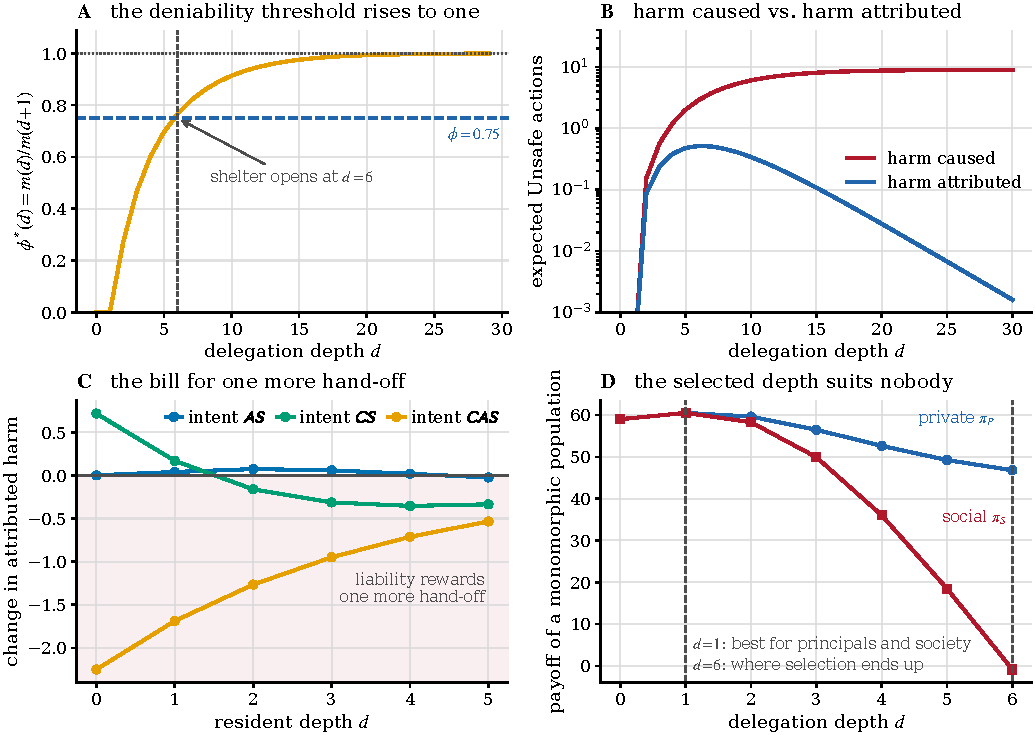
\includegraphics[width=\linewidth]{figures/fig03_shelter.pdf}
\caption{\textbf{Depth as a liability shelter.}
\textbf{(A)}~The deniability threshold $\phi^{*}(d)=m(d)/m(d{+}1)$ rises towards
one because realised harm saturates, so any attribution retention below one is
eventually below the threshold; at $\phi=0.75$ the shelter opens at six
hand-offs. \textbf{(B)}~Beyond that depth, realised harm still climbs towards
its ceiling while attributed harm falls geometrically. \textbf{(C)}~What one
more hand-off adds to the principal's bill. Where the curve is negative,
liability rewards delegation instead of taxing it. \textbf{(D)}~Private and
social payoff of a monomorphic population by depth. Selection ends at the
ceiling, which is worse for the principals than one hand-off and much worse for
everybody else.}
\label{fig:shelter}
\end{figure}

\subsection{Neither mechanism is dangerous alone}
\label{sec:decomposition}

The two mechanisms can be switched off independently: $\varepsilon=0$ removes
erosion and $\phi=1$ removes attenuated attribution. Crossing them gives a
$2\times2$ design whose four cells are reported in
Table~\ref{tab:decomposition} and Figure~\ref{fig:decomposition}.

Starting from a race that is already safe, erosion alone raises the long-run
unsafe frequency to $0.018$ and attenuated attribution alone to $0.012$. An
additive reading predicts $0.030$ when both are present. The measured value is
$0.322$. The interaction, $+0.293$, is $91\%$ of the joint effect, and the same
picture appears under the replicator reading, where the interaction is $+0.331$.

The mechanism behind the interaction is visible in the second panel of
Figure~\ref{fig:decomposition}, and it is not what one would guess. Under full
pass-through, erosion is a private cost, and the population responds to it by
\emph{shortening} its chains: mean depth falls from $6.00$ to $1.99$. Erosion
is self-limiting when the principal is charged for it. Attenuated attribution
does not make behaviour worse at a given depth; it removes the response. With
$\phi=0.75$ the chains stay at the ceiling and the same erosion now acts over
six hand-offs instead of two.

A counterfactual makes the decomposition exact. Scoring the pass-through
population with the per-layer harm matrix -- the same designs, charged
differently -- leaves the unsafe frequency at $0.018$, unchanged to nine
decimal places, because the behaviour of a given design does not depend on who
pays for it. The whole of the remaining $+0.305$ is composition: which designs
the population comes to contain. The result is a caution about a natural
inference. Observing that deeper chains behave worse does not license the
conclusion that the harm comes from erosion, because in this model almost all
of it comes from the depth the market selects once erosion is no longer its
problem.

\begin{figure}[t]
\centering
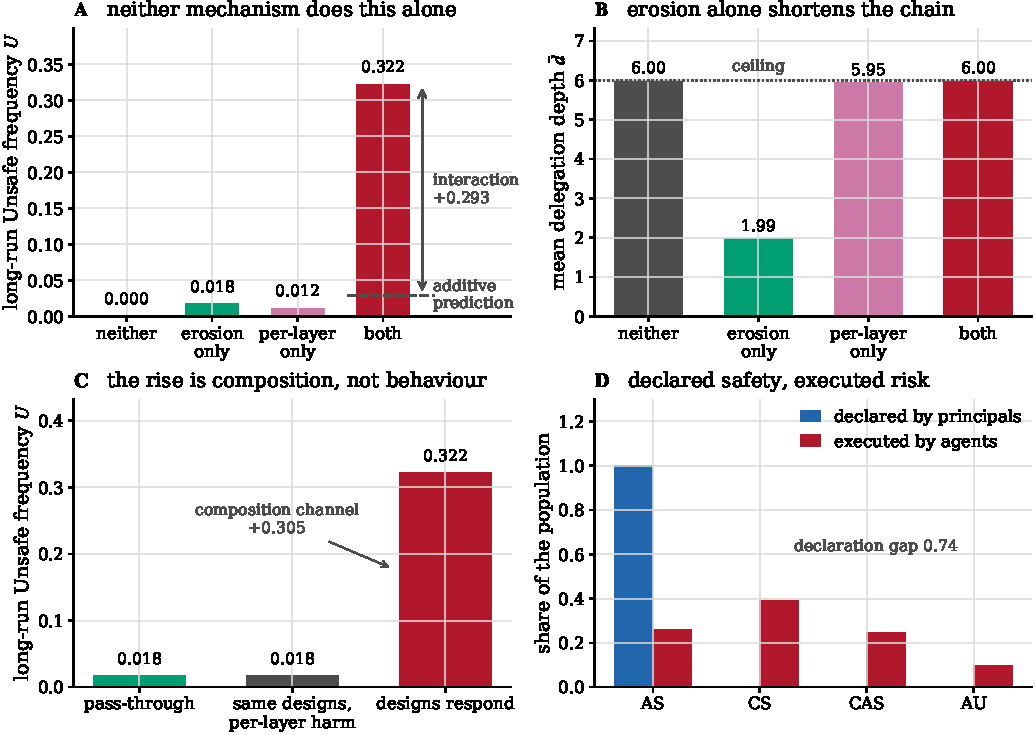
\includegraphics[width=\linewidth]{figures/fig04_decomposition.pdf}
\caption{\textbf{The two mechanisms, separately and together.}
\textbf{(A)}~Long-run unsafe frequency in the four cells of the $2\times2$. The
additive prediction from the two single-mechanism cells is $0.030$; the joint
outcome is $0.322$. \textbf{(B)}~Mean delegation depth in the same four cells.
Under pass-through the population answers erosion by shortening its chains;
per-layer attribution removes that answer and the ceiling binds.
\textbf{(C)}~Holding the pass-through population fixed and charging it the
per-layer bill changes nothing, so the entire rise is composition rather than
behaviour. \textbf{(D)}~In the joint cell every principal declares the safest
instruction and the population executes something else.}
\label{fig:decomposition}
\end{figure}

\subsection{The attribution--erosion plane}
\label{sec:plane}

Neither baseline value is doing the work. Figure~\ref{fig:plane} sweeps the
plane $(\varepsilon,\phi)$ on a $21\times21$ grid. The interaction index is
positive over $89\%$ of the interior and reaches $0.81$; the long-run unsafe
frequency reaches $0.995$ and the declaration gap $0.95$.

The second panel is the one to read for policy. Mean delegation depth splits
the plane along a frontier: below it the ceiling binds and chains are as long
as the technology allows, above it chains are short. The frontier runs
diagonally, so erosion and attribution are substitutes in producing long chains
-- a regime with faithful hand-offs tolerates much weaker attribution before
the ceiling binds, and a regime with strong attribution tolerates much noisier
hand-offs.

\begin{figure}[t]
\centering
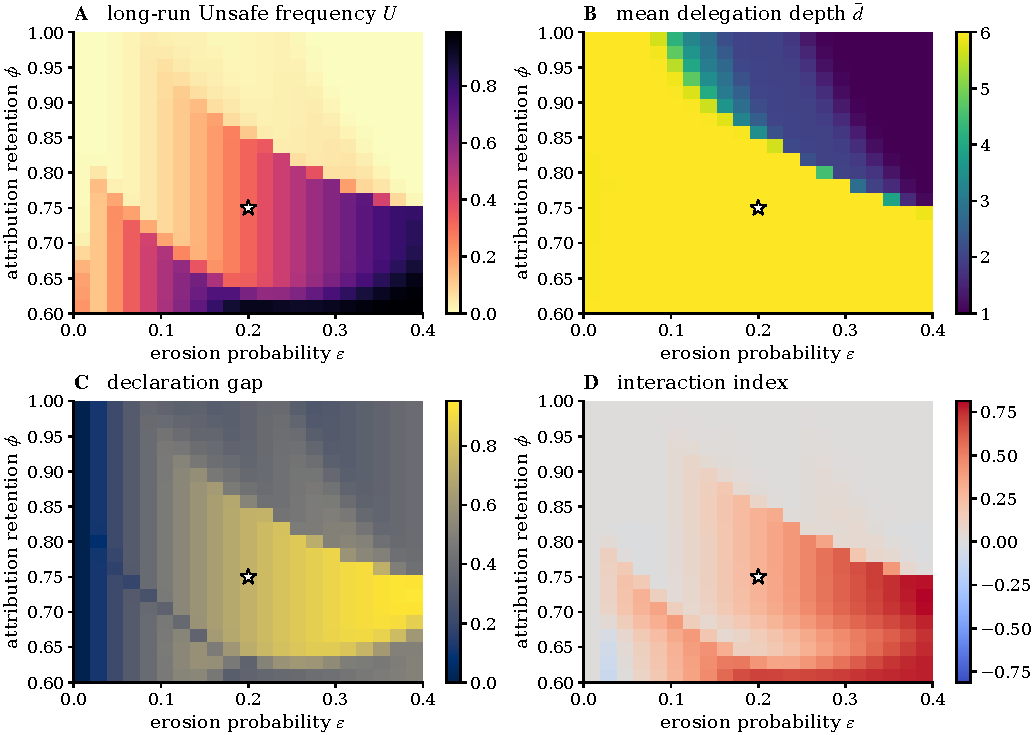
\includegraphics[width=\linewidth]{figures/fig05_plane.pdf}
\caption{\textbf{The attribution--erosion plane.} Long-run unsafe frequency
\textbf{(A)}, mean delegation depth \textbf{(B)}, declaration gap \textbf{(C)}
and interaction index \textbf{(D)} over a $21\times21$ grid; the star marks the
baseline. Chains are at the ceiling throughout the yellow region of
\textbf{(B)}, and the frontier that bounds it is diagonal: attribution and
transmission fidelity substitute for each other in keeping chains short.}
\label{fig:plane}
\end{figure}

\subsection{Declared safety and executed safety}
\label{sec:declaration}

At the baseline the population is monomorphic on the design $\AS{}@6$: every
principal issues the safest available instruction and every principal runs a
six-hand-off chain. What is executed is another matter. The realised mixture is
$26\%$ \AS{}, $39\%$ \CS{}, $25\%$ \CAS{} and $10\%$ \AU{}, and the total
variation distance between what is declared and what is executed is $0.74$.
Social payoff falls from $68.0$ in the baseline cell to $-0.8$.

The equilibrium is easy to misread as bad faith, and it is not. Every principal
is issuing the strongest safety instruction available to it, and doing so is a
best response: over-specification is how a principal compensates for a chain
that will erode whatever it is told. What the equilibrium shows is that a
declaration made at the top of a long chain carries almost no information about
the behaviour at the bottom of it. Any governance instrument that reads
declarations -- self-attestation, model cards, published policies -- is reading
a quantity that the model predicts will be maximally safe regardless of the
ecosystem it describes.

\subsection{What the instruments do}
\label{sec:instruments}

Four instruments act at different points of the chain: raise the attribution
retention $\phi$ towards pass-through; cap the permitted chain length at
$\bar D$; make every hand-off more faithful, multiplying $\varepsilon$ by a
factor $\rho$; or insert one check of strength $\alpha$ at a chosen layer.
Figure~\ref{fig:instruments} applies each to the same baseline.

\paragraph{Attribution is a threshold, not a dial.}
Raising $\phi$ from $0.75$ does nothing at all until $\phi=0.86$, where mean
depth falls from $5.92$ to $3.45$ and the unsafe frequency from $0.314$ to
$0.103$; by $\phi=0.99$ the outcome is the pass-through outcome. The location of
the jump is close to the closed form implied by Corollary~\ref{cor:failure},
$\phi_{c}=(L_{c}/L)^{1/D}=0.830$, the residual gap being the extra harm that
erosion contributes at depth. Partial pass-through buys very little: at
$\phi=0.85$, which returns $85\%$ of responsibility at each of six layers and
therefore $38\%$ overall, the ecosystem is still at $0.314$.

\paragraph{A ceiling buys safety and welfare at once.}
The depth ceiling is the only instrument here that is monotone in its own
strength and improves both objectives together. A ceiling of one hand-off
removes the unsafe behaviour entirely and lifts social payoff from $-0.8$ to
$60.5$; a ceiling of two leaves $0.018$ and $58.3$. The reason it works is that
the ceiling is the constraint the shelter theorem leaves standing when
attribution cannot be made exact.

\paragraph{Fidelity is not monotone.}
Attestation improves matters over most of its range, from $0.322$ at
$\rho=1$ down to $0.032$ at $\rho=0.35$, and then reverses: at $\rho=0.20$ the
unsafe frequency is back up to $0.239$. The cause is the intent margin.
Over-specification was an equilibrium response to erosion; once hand-offs are
faithful enough, issuing \CS{} rather than \AS{} becomes the better reply, and
\CS{} eroding into \CAS{} is far more damaging than \AS{} eroding into \CS{}.
A partial fidelity improvement can therefore leave the ecosystem worse off than
no improvement at all. The same reversal appears in the audit-placement sweep at
full strength, and for the same reason; at half strength, where the intent
margin does not flip, the sweep is monotone.

\paragraph{Check late, not early.}
For a fixed design the ordering is unambiguous.

\begin{proposition}[Audit placement]
\label{prop:audit}
Under a kernel satisfying the hypothesis of Proposition~\ref{prop:monotone},
the realised harm of a depth-$d$ chain carrying one check of strength $\alpha$
at layer $k$ is non-increasing in $k$.
\end{proposition}

\begin{proof}
The executed law is $\alpha M^{d-k}(s,\cdot)+(1-\alpha)M^{d}(s,\cdot)$, and by
Proposition~\ref{prop:monotone} the expected harm under $M^{j}$ is
non-decreasing in $j$. Increasing $k$ decreases $d-k$, hence decreases the first
term and leaves the second unchanged.
\end{proof}

In the equilibrium the effect is large: the same check is worth a factor of
$18$ more at the agent that acts than at the principal, $0.018$ against
$0.322$. Checking the specification a party \emph{received} tells you little
about what will be done with it several hand-offs later.

\paragraph{Which instrument is cheapest.}
Asking each instrument for the same target, a long-run unsafe frequency of at
most $0.05$, and scoring it by the social payoff it delivers there
(Figure~\ref{fig:frontier}B): attestation reaches the target at $58.7$, the
depth ceiling at $58.3$, a punitive liability at $56.2$ and pass-through at
$53.5$. The ranking is close enough that we would not press it, but the
qualitative message is not: raising the liability level is the least efficient
of the four, because it acts on a margin -- how much harm costs -- that
depth has already discounted.

\begin{figure}[t]
\centering
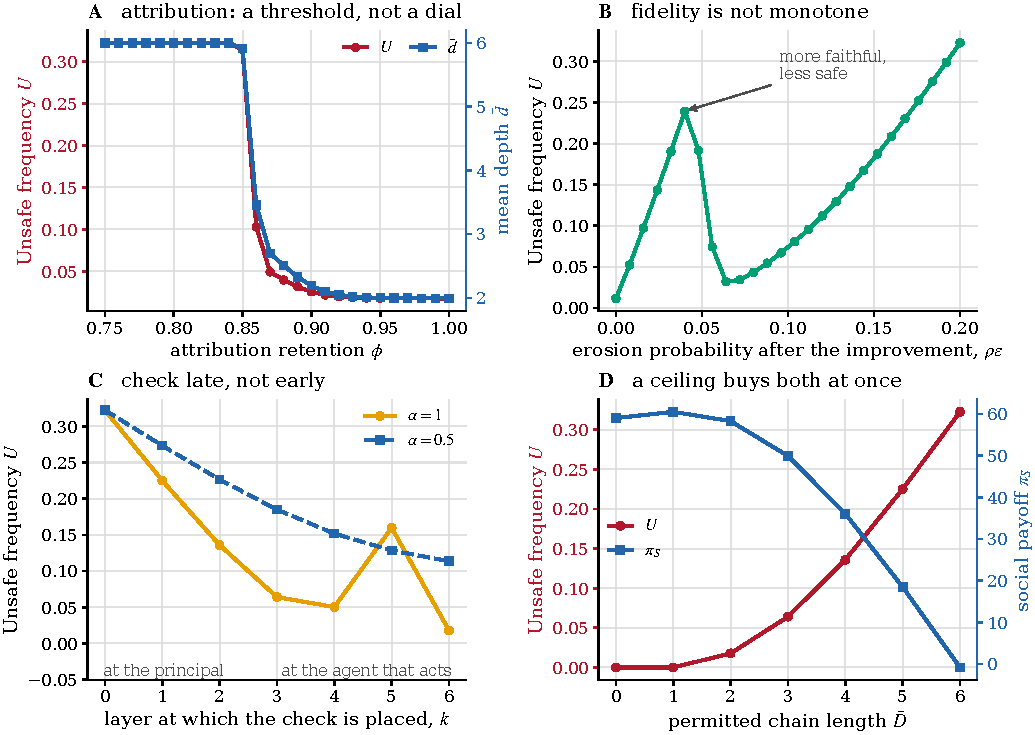
\includegraphics[width=\linewidth]{figures/fig06_instruments.pdf}
\caption{\textbf{Four instruments.}
\textbf{(A)}~Restoring attribution has a threshold at $\phi=0.86$ and does
almost nothing below it. \textbf{(B)}~Making every hand-off more faithful is not
monotone: the marked point is safer than settings with less erosion.
\textbf{(C)}~One check, moved down the chain. Late placement dominates; the
non-monotonicity at full strength is the intent margin flipping, and it is
absent at half strength. \textbf{(D)}~A ceiling on chain length improves safety
and welfare together.}
\label{fig:instruments}
\end{figure}

\begin{figure}[t]
\centering
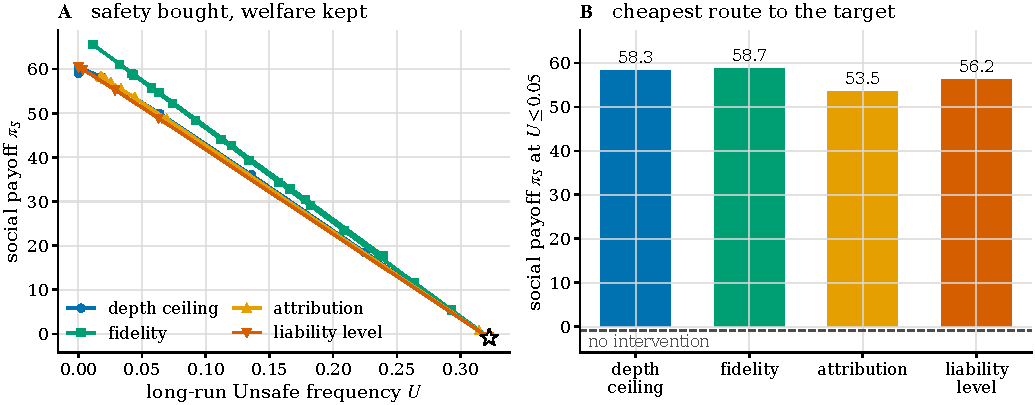
\includegraphics[width=\linewidth]{figures/fig07_frontier.pdf}
\caption{\textbf{What each instrument costs.} \textbf{(A)}~The frontier each
instrument traces in the plane of social payoff against long-run unsafe
frequency, starting from the untreated baseline (star). \textbf{(B)}~Social
payoff at the weakest setting of each instrument that reaches an unsafe
frequency of $0.05$. Raising the liability level is the least efficient route,
because depth has already discounted the margin it acts on.}
\label{fig:frontier}
\end{figure}

\subsection{Robustness}
\label{sec:robustness}

The $2\times2$ was recomputed across $43$ parameter cells: the prize and the
private setback risk of the race, both readings of what a setback destroys, the
organisational benefit and the coordination cost of a taller chain, the
population size, the selection intensity, the depth ceiling, the liability
level, and the choice between the finite-population and replicator readings.
The interaction is positive in $88\%$ of them, with median $+0.292$ and
interquartile range $[0.242,0.297]$; the median interaction share is $0.91$.
The mean delegation depth is higher under per-layer attribution than under
pass-through in every single cell. The negative cells are all in the
prize-and-risk sweep and are ceiling effects, where the joint outcome is already
at or near an unsafe frequency of one and cannot show a further increase.

The drift kernel is the one dimension along which the result genuinely changes,
and the direction is instructive (Figure~\ref{fig:robustness}B). Replacing
graded erosion by \emph{collapse}, in which a lost specification is replaced by
the unconditionally unsafe design rather than by the next rung down, all but
eliminates the effect: the joint cell falls to $3\times10^{-5}$ and mean depth
to $0.0002$. Delegation simply does not happen, because a chain that fails
catastrophically is one whose principal will not build it. Replacing graded
erosion by \emph{uniform} noise, which has the same spectral gap but no
direction, makes matters worse rather than better, with a joint cell of $0.517$.
The dangerous property of a hand-off is therefore not that it is biased but
that it degrades gracefully. A specification that fails loudly deters the
delegation that would have caused the harm; one that fails quietly does not.

\begin{figure}[t]
\centering

\includegraphics[width=\linewidth]{figures/fig08_robustness.pdf}
\caption{\textbf{Robustness.}
\textbf{(A)}~The interaction index across every sweep; each dot is one
parameter cell. \textbf{(B)}~Drift kernels. Graceful erosion produces the
cascade; catastrophic erosion deters delegation altogether; undirected noise is
worse than graded erosion, so the effect is not about the direction of the
slippage. \textbf{(C)}~The small-mutation limit against the full
mutation-selection chain on a reduced design space. \textbf{(D)}~Long-run
unsafe frequency against the effective liability at four attribution
retentions; a lower $\phi$ shifts the whole curve rather than tilting it.}
\label{fig:robustness}
\end{figure}

\section{Discussion}
\label{sec:discussion}

The model says something specific about where the governance of agentic systems
is currently pointed. Almost all of the instruments now being built read or act
at the two ends of a chain: evaluations and safety training at the model, and
liability, disclosure and procurement rules at the deploying principal. Both
ends are exactly where the model says the leverage is weakest.

At the principal end, Theorem~\ref{thm:shelter} says that a liability rule
written in terms of what a principal is responsible for has a depth beyond
which it stops binding, and Corollary~\ref{cor:failure} says where that depth
is. Raising the penalty does not move the failure depth much, because it enters
logarithmically; restoring attribution does, because it enters through
$\log\phi$. The practical form of that observation is unwelcome for a
regulator: partial pass-through is worth very little. Recovering $85\%$ of
responsibility at each of six hand-offs recovers $38\%$ overall and, in our
baseline, changes nothing at all.

At the model end, the declaration result says that a safety commitment issued at
the top of a long chain is close to uninformative about the ecosystem below it,
and not because anyone is lying. In the baseline equilibrium the declaration is
as strong as the language permits and the behaviour is $74\%$ different from it.
An evaluation regime that scores what a principal says, or scores a model in
isolation, is measuring a quantity that the model predicts will look good
precisely when the chain is long enough for it not to matter.

That leaves two instruments with real leverage, and they are the two least
discussed. The first is a limit on delegation depth. It is the constraint the
shelter theorem leaves standing, it is monotone in its own strength, and in our
baseline it improves welfare and safety simultaneously, which none of the
others do. The second is verification placed at the point of action rather than
at the point of instruction: a check of fixed strength is worth eighteen times
more at the agent that acts than at the principal that spoke.

The non-monotonicity result deserves its own caution. We find that making
hand-offs more faithful can raise realised harm, because the over-specification
that erosion had forced becomes unnecessary and the population relaxes its
declared intent by one clause, and a clause dropped from \CS{} costs far more
than a clause dropped from \AS{}. The general form of the caution is familiar
from other equilibrium settings: a partial fix to a friction that agents had
been compensating for can be worse than no fix, and the sign of the effect
cannot be read off the mechanism. In this model, only the instruments acting on
the incentive to delegate are monotone.

Finally, the kernel comparison suggests a design principle that does not come
from the liability literature at all. A specification that degrades gracefully
is more dangerous than one that fails loudly, because graceful degradation lets
a principal build a chain whose failures it never sees. Systems whose
specifications fail closed, refusing rather than approximating when a clause is
lost, restore the private cost of depth that per-layer attribution removes.

\section{Limitations}
\label{sec:limitations}

The interaction layer is a stylised two-player race with four reduced
strategies, inherited deliberately and without modification
from~\citet{domingos2026falling}. It is not a model of any deployed system, and the
absolute numbers should be read as the behaviour of that game rather than of a
market.

The erosion kernel is exogenous. We describe how a population behaves under a
given transmission technology and not how the technology itself is selected;
a model in which providers compete on fidelity would let $\varepsilon$
co-evolve with $d$, and the non-monotonicity in Section~\ref{sec:instruments}
suggests that the outcome would not be a simple race to the top. Our chains are
also linear, whereas real agentic systems branch, and a branching chain
aggregates several eroded specifications rather than one.

Geometric attribution is a modelling choice. It is the natural formalisation of
per-layer liability, in which each intermediary absorbs a fixed share, but real
attribution regimes are lumpier: a single identifiable intermediary may absorb
everything, or a strict pass-through rule may hold at some depths and not at
others. What the model requires is only that attribution be non-increasing in
depth and that it fall strictly at least sometimes;
Theorem~\ref{thm:shelter} needs $\phi^{d}m(d)\to 0$, which any
geometrically-bounded attribution rule delivers. A rule that floors attribution
at a positive constant $\phi_{\min}>0$ would cap the shelter, and locating the
floor at which the shelter closes is a natural next step.

Finally, the harm scale $h$ enters the social functional and therefore the
welfare comparisons, and we do not know it. We have kept the primary outcome,
the long-run unsafe frequency, free of welfare weights for that reason, and we
report social payoffs only for comparisons at a fixed $h$.

\section{Conclusion}
\label{sec:conclusion}

Delegation depth is not neutral plumbing between a principal and an action. It
erodes the specification geometrically and it dilutes the attributed harm
geometrically, and because the second effect is unbounded while the first
saturates, depth is a liability shelter that no level of liability closes. What
makes the combination dangerous is not either mechanism but the loss of a
response: a principal who is charged for what its chain does answers unreliable
hand-offs by keeping the chain short, and per-layer attribution is precisely
what stops it. In our baseline that lost response accounts for $91\%$ of the
damage, and it produces an equilibrium in which every principal issues the
safest instruction available and the ecosystem executes something $74\%$
different.

The instruments that follow are not the ones currently receiving attention.
Limiting how many hand-offs may separate an instruction from an action, and
verifying specifications at the agent that acts rather than at the party that
spoke, are the two levers that behave predictably in this model. Restoring
attribution works, but only when it is nearly complete; raising penalties works
least of all, because depth has already discounted the margin they act on.

\section*{Data and code availability}

All results are deterministic given the seed used for the replicator start
measure. Code, generated tables and the figure pipeline are available at
\texttt{github.com/\textless user\textgreater/delegation-cascade}.

\bibliographystyle{unsrtnat}
\bibliography{refs}

\end{document}
